% Created 2012-09-01 Sat 14:02
\documentclass[11pt]{article}
\usepackage[utf8]{inputenc}
\usepackage[T1]{fontenc}
\usepackage{fixltx2e}
\usepackage{graphicx}
\usepackage{longtable}
\usepackage{float}
\usepackage{wrapfig}
\usepackage{soul}
\usepackage{textcomp}
\usepackage{marvosym}
\usepackage{wasysym}
\usepackage{latexsym}
\usepackage{amssymb}
\usepackage{hyperref}
\tolerance=1000
\providecommand{\alert}[1]{\textbf{#1}}

\title{Tutorial: An Efficient Algorithm for Easy-First Non-Directional Dependency Parsing -- writing the code}
\author{Aviad Reich}
\date{2012-07-21 Sat}
\hypersetup{
  pdfkeywords={},
  pdfsubject={},
  pdfcreator={Emacs Org-mode version 7.8.09}}

\begin{document}

\maketitle

\setcounter{tocdepth}{3}
\tableofcontents
\vspace*{1cm}


\section{How to contribute to this document}
\label{sec-1}

  
\subsection{All formats}
\label{sec-1-1}

   This document exists in XHTML, latex, text and org-mode
   versions. Editing the first three is straightforward, but will force
   all future contributors (if such will exist) to use the same
   version/format, since this will break the compatibility of the
   different formats. Do this only if you're sure the future contributors
   will be OK with it, or you know they will not exist (for example: you
   are now completing the document). If you have done so, be sure to
   either label the other versions as outdated/irrelevant, or simply
   delete them.
\subsection{OPTION: Using Emacs' org-mode}
\label{sec-1-2}

   Another option is to edit the text file `tutorial.org' in you favorite
   text editor. If you ignore lines 5-15, it's pretty much
   straightforward to understand the usage: 
   The number of left-aligned `*' before a line determine it's `depth' in
   the document (more is deeper), and elements are automatically nested in
   the immediate higher level item. 

   if you want $\TeX{}$, or $\LaTeX$,
   include its code inside adjacent dollar signs: \\
   \texttt{\$[latex code here]\$}.
   Just look at `tutorial.org' for examples.

   To use the other many wonderful, yet simple to use, features of
   org-mode, like auto-numbering of items, footnotes and others, 
   it's recommended you read the \href{http://orgmode.org/}{orgmode website} and the (relevant) \href{http://orgmode.org/org-mode-documentation.html}{docs},
   or the tutorial that comes with it as part of Emacs, or \href{http://orgmode.org/worg/org-tutorials/}{these tutorials}.

\begin{description}
\item[TODOs] When (if..) you complete an item that is marked as a red
             `TODO', just delete the word `TODO' from the \texttt{org}
             file. Once a whole section is done, delete the topmost
             `TODO', and the `[x/x]' after the section name, so they will
             no longer be displayed. You could optionally move the cursor
             to the line with a `TODO' and press Ctrl-c Ctrl-t to mark
             that item as done (and add a timestamp).  An additional
             Ctrl-c Ctrl-t will remove the TODO altogether.
\end{description}


\begin{description}
\item[Exporting] To export to HTML, tex and text once you're done, open
             Emacs (you  know where to get it), press Ctrl-x Ctrl-f
             and type the path to the file. Then, press Ctrl-c
             Ctrl-e h (for HTML), Ctrl-c Ctrl-e p (for pdf), Ctrl-c
             Ctrl-e l (for latex), Ctrl-c Ctrl-e u (for unicode
             text, a for ascii). Many other export format exist -
             you'll find it in the ``Emacs-style popup''
             window. \\
             \textbf{MAKE SURE YOU EXPORT IN ALL FORMATS ONCE YOU'RE              DONE, SO COMPATIBILITY IS MAINTAINED.}
\end{description}

As this is written (August 2012), I care about this document, and
would be happy to extend my help if it's wanted. To email me use the
first 3 letters of `Aviad', followed by a dot (`.') and the
first 3 of `Reich'. Then mail me at: \texttt{[what-you-got]@gmail.com}.

Additionally, there is a github repo:
\href{https://github.com/lxmonk/NLP12-Easyfirst_tutorial}{https://github.com/lxmonk/NLP12-Easyfirst\_tutorial}, that you can clone
or fork. If you do, and you've created a new one - change this
address. Otherwise, let me know and I'll update.
\section{\textbf{TODO} An intro to dep parsing [0/3]}
\label{sec-2}
\subsection{\textbf{TODO} Formats of the data}
\label{sec-2-1}
\subsection{\textbf{TODO} Example sentences}
\label{sec-2-2}
\subsection{\textbf{TODO} Rendering of trees in text and graphically}
\label{sec-2-3}
\section{\textbf{TODO} Intro to dep parsing using transition based parsing [0/2]}
\label{sec-3}
\subsection{\textbf{TODO} How shift reduce works}
\label{sec-3-1}
\subsection{\textbf{TODO} Turning a tree into a sequence of shift reduce transitions}
\label{sec-3-2}
\section{\textbf{TODO} Malt like parsing [0/2]}
\label{sec-4}
\subsection{\textbf{TODO} Training a classifier to learn which transition is best at each step}
\label{sec-4-1}
\subsection{\textbf{TODO} Typical features used for malt}
\label{sec-4-2}
\section{\textbf{TODO} Evaluation methods for dep parsing}
\label{sec-5}
\section{\textbf{TODO} Evaluation of a demo malt parser}
\label{sec-6}
\section{Easy First}
\label{sec-7}

  
\subsection{Read the paper}
\label{sec-7-1}


The article: \\
\textbf{Easy First Dependency Parsing of Modern Hebrew}, \\
   Yoav Goldberg and Michael Elhadad, \\
   \emph{SPMRL 2010 (NAACL Workshop on Statistical Parsing of    Morphologically-rich Languages)}


It can be obtained from \href{http://www.cs.bgu.ac.il/~yoavg/publications/naacl2010dep.pdf}{Yoav Goldberg's BGU webpage}, or at the acm
website: 
\href{http://dl.acm.org/citation.cfm?id=1857999.1858114}{http://dl.acm.org/citation.cfm?id=1857999.1858114}.


   
\subsection{Quiz on the paper}
\label{sec-7-2}
\subsubsection{Introduction and Easy-First}
\label{sec-7-2-1}


\begin{enumerate}
\item From the article (pg. 1): \\
``Current dependency parsers can be categorized
     into three families: \textbf{local-and-greedy transition-based parsers}
     (e.g., MALTPARSER (Nivre et al., 
     2006)), \textbf{globally optimized graph-based parsers}
     (e.g., MST P ARSER (McDonald et al., 2005)), and
     \textbf{hybrid systems} (e.g., (Sagae and Lavie, 2006b;
     Nivre and McDonald, 2008)), which combine the
     output of various parsers into a new and improved
     parse, and \textbf{which are orthogonal to our approach}.''  (no emphasis   
   in the original text) \\
   \underline{Who is orthogonal to the authors' approach? Why?} \\
\begin{description}
\item[a] Local-and-greedy transition-based parsers
\item[b] Globally optimized graph-based parsers
\item[c] Hybrid systems
\item[d] All of the above
\item[e] None of the above
\end{description}
\item According to the article, what are the shortcomings of
   transition-based parsers? Which of these have been addressed by the
   easy-first parser? How?
\item One might claim that transition-based parsers suffer from an
   imbalance, in relation to the knowledge they have about the
   sentence as it's being parsed. How might easy-first help to mend
   this?
\item Why are transition-based parsers often restricted to only a limited
   look-ahead window?
\item When will we prefer a globally optimized graph-based parser over a
   transition-based parser? When would a transition-based one be more
   appropriate?
\item The article states that easy-first is a greedy algorithm. What are
   the benefits of this fact?
\item How are transition-based parsers different than humans when
   dependency-parsing a sentence?
\item Do humans annotate a sentence in a way similar to graph-based
   parsers?
\item Of the three parser classes (transition, graph-based and
   easy-first), which is the most similar to a human's way of
   annotating a sentence?
\item In your opinion, is being similar to the human way of parsing a
    sentence a positive or a negative approach to the problem? Why?
\end{enumerate}
\subsubsection{Parsing Algorithm}
\label{sec-7-2-2}


\begin{enumerate}
\item Look at figure 1 in the article. In each step, how is the action
    to be performed chosen?
\item In step 1 (figure 1), if the bold number \textbf{403} was instead 136,
   what action would have been performed?
\item What is the range of values for the arc ``brown --> fox'', assuming
   all others remain unchanged, that will lead to the same parse tree?
   What is the range for the arcs ``a --> brown'' and ``joy --> with''
   that will lead to the same parse tree?
\item Assuming the \textbf{difficulty} of choosing an action is measured by the
   difference between the two highest arc's score. On which step was
   making this decision hardest? Can you ``feel'' this difficulty trying
   to parse the sentence yourself?
\item Algorithm 1.1 is identical to algorithm 1 (see below), but in it, line 3 is \textbf{changed} to
   $pending = p_{1} \ldots p_{n-1} \leftarrow w_{1} \ldots w_{n-1}$.
   What will be the first step in parsing the sentence ``a brown fox
   jumped with joy'' in which the two algorithms will diverge? (hint:
   use figure 1) 
   In general, what will this change cause? \\
   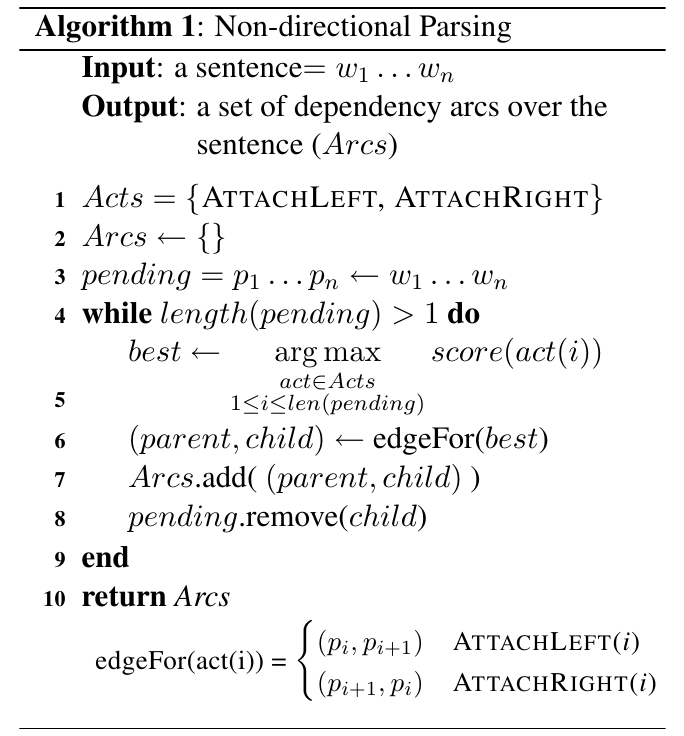
\includegraphics[width=.9\linewidth]{images/Algorithm1.png}]] \\
\item What does the function EdgeFor do? How?
\item Write the loop from line 5 in python.
\item Can you find this loop in the file \hyperref[sec-9-1]{easyfirst.py}? 
\begin{description}
\item[hint 1] the variables in lines 174,175 are never used, and can
               be safely removed from the \texttt{train} function).\\
\item[hint 2] \texttt{In [1]: zip(range(10), range(10)[1:])} \\ 
\texttt{Out[1]: [(0, 1), (1, 2), (2, 3), (3, 4), (4, 5), (5, 6), (6, 7), (7, 8), (8, 9)]}
\end{description}
\item In line 5, where is $score(act(i))$ taken from?
\end{enumerate}
\subsubsection{Learning Algorithm and Feature Representation}
\label{sec-7-2-3}

    see \hyperref[sec-7-2-5]{Perceptron Classifier}
    
\subsubsection{Computational Complexity and Efficient Implementation}
\label{sec-7-2-4}

     
\begin{enumerate}
\item From the article (pg. 5): \\
``The parsing algorithm (Algorithm 1) begins with
   $n + 1$ disjoint structures (the words of the sentence +
   ROOT symbol), and terminates with one connected
   structure. Each iteration of the main loop connects
   two structures and removes one of them, and so the
   loop repeats for exactly $n$ times.
   The $\arg\max$ in line 5 selects the maximal scoring
   action/location pair. At iteration $i$, there are $n - 1$
   locations to choose from, and a naive computation of
   the $\arg\max$ is $O(n)$, resulting in an $O(n^{2})$ algorithm.''\\
   Is the algorithm really $O(n^{2})$? \\
   \textbf{Why? What is the non-naive computation?}
\item From the article (pg. 5: footnote 4): \\
``Indeed, in our implementation we do not use a heap, and
   opt instead to find the argmax using a simple O(n) max
   operation. This $O(n^2)$ algorithm is faster in practice than the heap 
   based one, as both are dominated by the $O(n)$ feature extraction,
   while the cost of the $O(n)$ max calculation is negligible 
   compared to the constants involved in heap maintenance.'' \\
   \textbf{a) What should have been the complexity using the heap?} \\
   \textbf{b) Can you think of a situation in which a heap should be used in the    implementation?}
\item Beam search parsers are only mentioned in Table 1 in the
   article, and the quoted article was published 2 years prior. Do you
   think this might imply at the identity of the identity of the
   editor/reviewers of the NAACL article (this one)? :)
\end{enumerate}

    
\subsubsection{\textbf{TODO} \label{Perceptron-Classifier}Perceptron Classifier}
\label{sec-7-2-5}

    
\subsubsection{\label{Cython}Cython}
\label{sec-7-2-6}

\begin{enumerate}
\item First, if you are not yet familiar with \href{http://cython.org}{Cython}, it's highly
      recommended you read the \href{http://docs.cython.org/}{docs} first, or minimally (and
      reasonably) \href{http://conference.scipy.org/proceedings/SciPy2009/paper_1/full_text.pdf}{the tutorial (pdf)}. A \emph{very} minimal \hyperref[sec-8]{Cython Primer} is given
      below.
\item In the file \hyperref[sec-9-2]{ml.pyx} below, what classes are created?
\item Which of them are python-only? Why?
\item There are several ``data'' classes: \texttt{DoublesArr},
      \texttt{MulticlassModel}, \texttt{MulticlassParamData}, \texttt{MultitronParameters},
      \texttt{ParamData}, \texttt{PerceptronParameters}. What is each of them used for?
\item Where in the code is the Perceptron initialized? What are the
      initial values?
\item Where is the learning (adjustment of parameters) happening?
\item In line 518, the \texttt{score} function is defined. Follow the code,
      and answer these questions:
      a) How is the score calculated?
      b) When will the \texttt{except} clause (lines 528-529) be executed?
      c) Can you re-write the function using a functional (rather than
      the current imperative) style?
\end{enumerate}



    
  
\section{\label{Cython-Primer}Cython Primer}
\label{sec-8}

    From \href{https://en.wikipedia.org/wiki/Cython}{Wikipedia}: \\
    ``Cython is a programming language to simplify writing C and C++
    extension modules for the CPython Python runtime.\footnote{DEFINITION NOT FOUND: 3 } Strictly
    speaking, Cython syntax is a superset of Python syntax
    additionally supporting: 
\begin{itemize}
\item Direct calling of C functions, or C++ functions/methods, from Cython code.
\item Strong typing of Cython variables, classes, and class attributes
      as C types.
\end{itemize}
    Cython compiles to C or C++ code rather than Python, and the
    result is used as a Python Extension Module or as a stand-alone
    application embedding the CPython runtime.''

    The importance of Cython in the implementation of the easy-first
    algorithm, is that it allows a fast and optimized version of
    python to be executed. This is not an accurate statement, but it
    suffices for this paper.

    The Cython code, is used to create the \texttt{ml} module, and is found
    in the file \texttt{ml.pyx}. This file is \textbf{compiled} to the file \texttt{ml.c},
    but for clarity, read the \texttt{.pyx} file, not the C one.

    If you have not read any of the links above, here is the bare
    minimum you need to know in order to read \texttt{ml.pyx}: 
\begin{enumerate}
\item \texttt{cimport} means `import from a C library.'
\item \texttt{cdef} means `define in C -- usually it'll be a function, a
       (python) class, or a variable definition, and will have a type.'
\item Types are declared. To declare (for example) a pointer to a
       double, either \texttt{cdef double* double\_ptr} or \texttt{<double *>        func(args)} is used.
\item \texttt{cpdef} means `this is defined in a way that will be accessible
       from both python and c.' In order to define a python-only
       function, the usual \texttt{def} applies.
\item A return type is declared for C functions. For example, \\
\texttt{cpdef object get\_scores(self,list features):} (taken from \texttt{ml.pyx} line 133) means: the
       function \texttt{get\_scores} is defined in both python and C. it will
       \textbf{return an object}, and will receive a \texttt{python list} type bound
       to the \texttt{features} variable. As in python, \texttt{self} means it's a method
\item \texttt{\_\_cinit\_\_} is the class constructor (python's \texttt{\_\_init\_\_}) when
       executed from C. Think of it as \texttt{\_\_init\_\_}.
\item \texttt{\_\_dealloc\_\_} is the class destructor.
\end{enumerate}
       
    
\section{Code}
\label{sec-9}
\subsection{\label{easyfirst.py}easyfirst.py:}
\label{sec-9-1}

\href{https://gist.github.com/3467275}{https://gist.github.com/3467275}
\subsection{\label{ml.pyx}ml.pyx:}
\label{sec-9-2}

\href{https://gist.github.com/3566683}{https://gist.github.com/3566683}

\end{document}